%% Estructura principal para un reporte de Trabajos intersemanales CIRCAE %%
\documentclass[a4paper]{IEEEtran} %tamaño del papel y el tipo de transcripción que será IEEE
\usepackage[utf8]{inputenc} %el tipo de codificación que incluye símbolos como la tilde
\usepackage[spanish]{babel} % hacemos que nuestro documentación vaya en español
\usepackage{cite} % citas bibliográficas
\usepackage{graphicx} %gráficos, usaremos solo .jpg o .png con estándares que ya veremos
\usepackage{subfigure}
\usepackage{url}
\usepackage{amsmath} 
\begin{document}

\title{WILKINSON POWER DIVIDER SIMULATION}
\author{Hanan Ronaldo Quispe Condori, CIRCAE Student Member}
\markboth{INFORME CIRCAE 2019-08-05-G1-P3-001}{} % Codigo del informe que corresponde a: semestre | mes | dia | numero de grupo con la G antepuesta | numero de proyecto con la P antepuesta | número de informe
\maketitle
\begin{abstract}
El divisor de potencia de Wilkinson es un dispositivo pasivo con todos sus puertos emparejados,no tiene perdidas cuando el puerto de entrada se excita y los puertos de salida estan aislados,esta simulacion imlementara un divisor de potencia para el rango de frecuencia de 0 a 2GHz.
\end{abstract}
\section{Problema}
La division de una señal de entrada en señales de salida equiamplitud y equifase se logra con un divisor tipo T o un divisor resistivo,pero estos presentan la limitacion de tan solo poseer un numero par de salidas, por ejemplo en caso se necesitaran usar 9 salidas, un divisor de 16 salidas tendria que ser utlizado, esto produciria disipación de potencia innecesaria,el divisor de potencia de Wilkinson soluciona este problema.
\begin{figure}
    \centering
        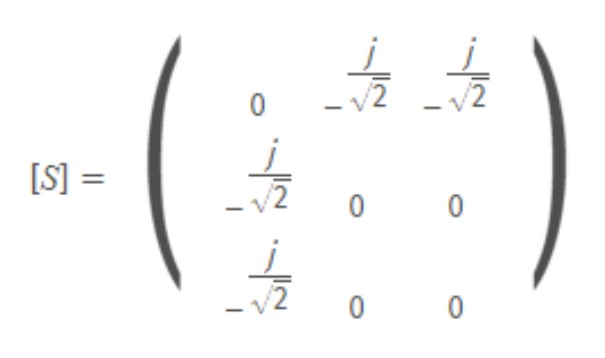
\includegraphics[width=8cm]{imagenes/img1}
        \caption{A gull}
        \label{fig E-field phase animation of a Wilkinson power divider.}
\end{figure}
%La bibliografía:
\bibliographystyle{ieeetr}
\bibliography{bibliografia}

\end{document}